\chapter{Introduction}

\section{Learning Technology}

% WHAT SHOULD GO HERE?
% Introduction to spaced repetition
% Survey of learning technologies used
% Gamification explained, stigma, some stuff about Skinner maybe?

\par Learning technology is becoming nearly universally used in classrooms, to the point where some teachers refer to it as "mandatory." Yet there is still a "great variation in university lecturers' use of technology," with some teachers not even ready to replace their overhead slides with Powerpoint \cite{BJET:BJET12051}.

\par We will address the different methodologies teachers use to integrate technology with the classroom, paying special attention to gamification techniques and spaced repetition.

\section{Definitions}

\subsection{Spaced Repetition}
\par Spaced repetition is a learning technique first coined by Dr. Paul Pimsleur in 1967 \cite{pimsleur1967memory}. Dr. Pimsleur noted the existence of a "forgetting curve." (See \textbf{\hyperref[fig:forgetting-curve]{Figure \ref*{fig:forgetting-curve}}}) The first moment a piece of information is learned, the subject is 100\% likely to be able to correctly recall it. However, as early as the first day after initially learning the information, the subject's retention rate of the information begins rapidly decaying. By reviewing the information, the retention rate is brought back to 100\%, and the subsequent decay of retention is substantially \textit{flattened}. That is, as students review information over time, it is encoded into their long-term memory, and they are less likely to forget it over a long period of time.

\begin{figure}[h]
	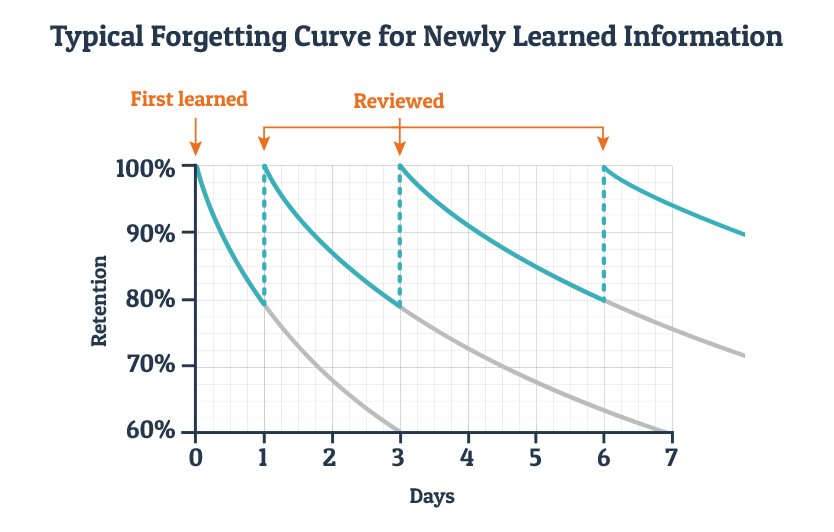
\includegraphics[width=1.0\linewidth]{figures/forgetting-curve}
	\caption{The "Forgetting Curve," as presented by Dr. Pimsleur in 1967. The y-axis represents the subject's likelihood of recalling a specific piece of information at the given time.}
	\label{fig:forgetting-curve}
\end{figure}

\par Dr. Pimsleur initially proposed spaced repetition as a technique solely for learning a new foreign language, but spaced repetition has been proven to be effective for any classroom setting. As Kang notes in \cite{fiske2016spaced}, it is intuitive that information needs to be practiced and reviewed over time to be fully integrated into a student's understanding, but Dr. Pimsleur's techniques provide a quantifiable, scientific schedule to maximize retention.

\par Kang et al. \cite{fiske2016spaced} also attempts to find the "Optimal Spacing Lag," or the optimal time between each review session for a particular piece of information after a long period. They find that this optimal spacing lag is around 10\% to 20\% of the time between initial introduction of the information and the test date. That is, if the test is 10 weeks away, even the oldest information should be reviewed with at most a 1-2 week delay in between review sessions.

\begin{figure}[h]
	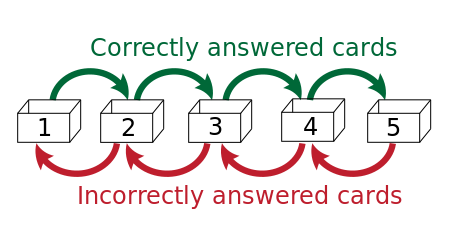
\includegraphics{figures/leitner}
	\caption{The Leitner system. If a student answers a flashcard correctly, it is moved to a higher-numbered box that is reviewed less frequently.}
	\label{fig:leitner}
\end{figure}

\par A simple example of spaced repetition is the Leitner system. Flashcards corresponding to the desired source material are organized into numbered boxes. (See \textbf{\hyperref[fig:leitner]{Figure \ref*{fig:leitner}}}). Each successive box is reviewed less frequently. That is, a student would review Box 1 twice per day, Box 2 once per day, Box 3 every 2 days, and so on. If a card is answered correctly, it is moved to a box that is reviewed less frequently. However, if the student answers incorrectly, the card is moved to a box that is reviewed more frequently.

\par Thus, tougher cards are reviewed more often, and cards the student knows will be reviewed less often. However, all cards are \textit{eventually} reviewed, and even cards that the student always answers correctly are reviewed in the long term.

\subsection{Gamification}
\par The term "gamification" first appeared in 2008 , but the concept wasn't known in the mainstream until 2011 with the advent of Foursquare \cite{Deterding:2011:GDE:2181037.2181040}. Foursquare is an app that takes the mundane concept of reviewing restaurants and finding new places to visit and turns it into an engaging, popular experience. Users of the app earn points for "checking in" at locations. This is a great example of gamification, which doesn't have an easy, exact definition. 

\par In Deterding's paper \cite{Deterding:2011:GDE:2181037.2181040}, they propose a categorical definition based on the concept of "gamefullness," which is the concept of presenting a systematic reward for a desired behavior.  
% TODO here: fill in section on gamification, include definition, some papers on different techniques and how it affects the brain.

%\subsection{Why College Classes?}
%\par \textit{Commit} was tested with classes at California Polytechnic State University to facilitate the creation of questions and evaluation of the application. While the app would work with any level of education from K-12 to higher education, using Cal Poly classes allowed us to easily create questions for classes that we had just taken

%\par Gamifying in education has several hurdles. Gamification tends to come with a negative stigma; teachers often feel that gamified services aren't as "serious" as other learning technologies. In addition, existing education gamification solutions have usability issues and are not accessible to students that don't have a background in videogames.

%[http://www.memorylifter.com/fileadmin/publications/Spacing_Effect_and_Mnemonic_Strategies.pdf]
